%!TEX root = ../Main.tex

\begin{figure}

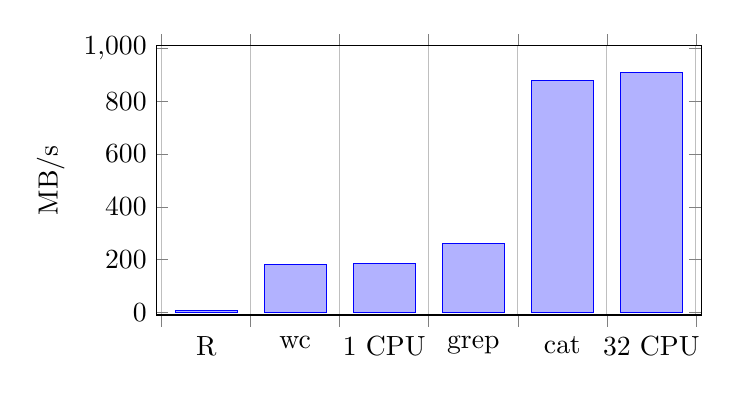
\begin{tikzpicture}
\begin{axis}[
	ylabel=MB/s,
  ymin=0, ymax=1000,
	enlargelimits=0.01,
	ybar interval=0.7,
  symbolic x coords={R, wc, 1 CPU, grep, cat, 32 CPU, end},
  width=8.5cm, height=5cm,
]
\addplot coordinates {(R,6.0) (wc,182.6) (1 CPU,186.6) (grep,261) (cat,878) (32 CPU,908) (end,0) };
% \addplot coordinates {(R,6.0) (wc,182.6) (CPU1,186.6) (grep,261) (wc -l,852) (cat,878) (Run 372,908) (Run 1,1029) (end,0) };

% \legend{MB/s}

\end{axis}
\end{tikzpicture}

\caption{Throughput comparisons of Icicle (1 CPU and 32 CPU) against existing R code and standard Unix utilities; higher is faster.}
\label{fig:bench:other}
\end{figure}

